\documentclass[10pt]{article}
\usepackage[utf8]{inputenc}
\usepackage[T1]{fontenc}
\usepackage{hyperref}
\hypersetup{colorlinks=true, linkcolor=blue, filecolor=magenta, urlcolor=cyan,}
\urlstyle{same}
\usepackage{graphicx}
\usepackage[export]{adjustbox}
\graphicspath{ {./images/} }
\usepackage{amsmath}
\usepackage{amsfonts}
\usepackage{amssymb}
\usepackage[version=4]{mhchem}
\usepackage{stmaryrd}
\usepackage{caption}

\title{Theory of "Hot" Photoluminescence from Drude Metals }

\author{Yonatan Sivan* and Yonatan Dubi}
\date{}


\begin{document}
\maketitle
\captionsetup{singlelinecheck=false}
Cite This: ACS Nano 2021, 15, 8724-8732\\
Read Online\\
Downloaded via BEN GURION UNIV OF THE NEGEV on September 1, 2024 at 12:48:44 (UTC). See \href{https://pubs.acs.org/sharingguidelines}{https://pubs.acs.org/sharingguidelines} for options on how to legitimately share published articles.

\begin{abstract}
We provide a complete quantitative theory for light emission from Drude metals under continuous wave illumination, based on our recently derived steady-state nonequilibrium electron distribution. We show that the electronic contribution to the emission exhibits a dependence on the emission frequency which is very similar to the energy dependence of the nonequilibrium distribution, and characterize different scenarios determining the measurable emission line shape. This enables the identification of experimentally 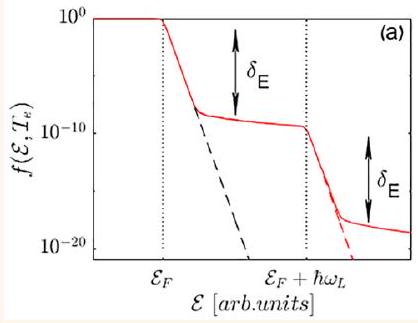
\includegraphics[max width=\textwidth, alt={}]{f97508c2-190d-403e-b38d-02344f5e51bf-1_323_418_930_1123} 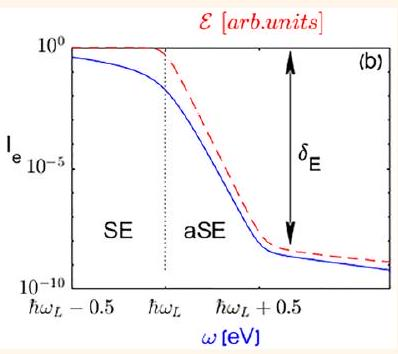
\includegraphics[max width=\textwidth, alt={}]{f97508c2-190d-403e-b38d-02344f5e51bf-1_354_398_901_1563} relevant situations, where the emission lineshapes deviate significantly from predictions based on the standard theory (namely, on the photonic density of states), and enables the differentiation between cases where the emission scales with the metal object surface or with its volume. We also provide an analytic description (which is absent from the literature) of the (polynomial) dependence of the metal emission on the electric field, its dependence on the pump laser frequency, and its nontrivial exponential dependence on the electron temperature, both for the Stokes and anti-Stokes regimes. Our results imply that the emission does not originate from either Fermion statistics (due to $e-e$ interactions), and even though one could have expected the emission to follow boson statistics due to involvement of photons (as in Planck's Black Body emission), it turns out that it deviates from that form as well. Finally, we resolve the arguments associated with the effects of electron and lattice temperatures on the emission, and which of them can be extracted from the anti-Stokes emission.
\end{abstract}

KEYWORDS: "Hot" photoluminescence, plasmonics, non-thermal electrons

\section*{INTRODUCTION}
The observation of emission of light from illuminated metal surfaces is over half a century old. ${ }^{1}$ In order to distinguish it from blackbody (BB) emission (also termed as photoluminescence, PL), this effect was coined as "hot" PL ${ }^{2}$ (meaning that it is due to nonthermal (aka "hot") electron distribution ${ }^{3}$ ) as secondary light emission or as inelastic light scattering. ${ }^{4,5}$ The emission process attracts an ongoing heated debate associated with its exact theoretical nature, ${ }^{2,4,6-9}$ partially because of the desire to explain the origin of the spectral background in surface enhanced Raman scattering (SERS); see discussion in ref 5 .\\
While the quantum yield of "hot" PL from metal surfaces is very small $\left(\sim 10^{-10}\right)$, ${ }^{1}$ subsequent studies showed that it can be significantly increased by roughening the surface ${ }^{10}$ or by considering metallic nanoparticles (NPs). ${ }^{11-13}$ This discovery impelled metal NP "hot" PL into applications in bioimaging as fluorescent markers, ${ }^{14-16}$ in optical recording, ${ }^{17}$ as means of monitoring chemical reactions, ${ }^{18,19}$ for spectroscopic mode mapping, ${ }^{20}$ and for thermometry. ${ }^{21-24}$

Parallel experimental studies were aimed at explaining various fundamental aspects of the problem, including the\\
characterization of the emission from NPs of different shapes, ${ }^{25-30}$ and the dependence of the Stokes emission (SE) and anti-Stokes emission (aSE) on parameters such as the laser (pump) frequency $\omega_{L}{ }^{4,5,29,31,32}$ temperature, and electric field. ${ }^{33}$ Other studies focused on the distinction between the effects of one ${ }^{16,21,29,33-35}$ and two ${ }^{14,36-39}$ photon absorption on the emission. A feature which has attracted a lot of attention has been the spectral shift between scattering and luminescence spectra (see, e.g., refs 10, 16, 27, 34-36, and 40-43)\\
While most work identified interband transitions as the source of luminescence, ${ }^{1,4,10,16,27,30,42,44}$ fewer works studied the contribution of intraband transitions to the "hot" PL, ${ }^{5,21,28,29,33-35}$ which might be weaker for short pump wavelengths but dominant for longer ones. Similarly, most

Received: January 28, 2021\\
Accepted: April 23, 2021\\
Published: April 27, 2021\\
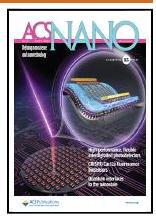
\includegraphics[max width=\textwidth, alt={}, center]{f97508c2-190d-403e-b38d-02344f5e51bf-1_216_156_2371_1807}\\
work was performed on gold nanoparticles (NPs), and only a few studies were dedicated to Ag NPs. In particular, some earlier work reported "hot" PL originating from interband transitions in silver films and colloids, $4,10,13,31,32,36$ but onephoton "hot" PL of silver nanoparticles which originates from intraband transitions was reported only in much fewer studies. ${ }^{29,33,45}$

Most importantly, in contrast to the large body of experimental work on plasmonic "hot" PL, there are surprisingly few comprehensive theoretical studies (see, e.g., refs $4,10,44$, and 46 ) so that our understanding of the underlying physics of the problem is limited. For example, the popular theory of ref 10 took into account the photonic aspect of the problem, namely, the enhancement of the absorption and emission (much like in the context of Purcell and Raman enhancement of molecules adjacent to metal nanoparticles ${ }^{47}$ ) due to volume and surface plasmon resonances; these aspects relate to the modification of the local density of photon states (LDOPS) due to structuring of the metal. The electronic part of the problem was treated in ref 10 partially, specifically employing an educated yet crude guess regarding the quantitative properties of the nonequilibrium electron distribution due to interband transitions. In other works, the electron system was assumed to follow a Fermi-Dirac distribution at a zero temperature ${ }^{48,49}$ while in other studies, ${ }^{4}$ this was done implicitly, by not accounting for the complete population in the first place. In other studies, thermal distributions at room temperature were adopted (e.g., as in refs 44 and 46)

In essentially all the other approaches, the electronic aspects of the problem were not accounted for at all. As a result, existing theoretical work provides only a partial, nonquantitative treatment of the practical aspects of "hot" PL. Specifically, essential features such as the dependence of the electron distribution on the laser frequency $\omega_{L}$ or the existence of anti-Stokes emission are not captured by these theories, and deviations of the emission line shape from the predictions of the standard Purcell theory could not be explained. Another confusion was related to the potential roles of the electron and phonon temperatures. ${ }^{43,50,51}$

One of the main reasons for the limitations mentioned above is that since "hot" PL is a property of the illuminated electronic system away from equilibrium, a full theoretical description requires knowledge of the electron nonequilibrium distribution. However, until recently, there was no reliable quantitative model for the steady-state electron nonequilibrium distribution in an illuminated metal that accounts for thermal and nonthermal effects on the same footing (i.e., a model that computes the electron nonequilibrium while allowing the electron and phonon temperatures to rise above the ambient temperature).

In refs 3 and 52, we employed a semiquantum Boltzmann model coupled with macroscopic equations for the total energy in the system (i.e., including, photons, electrons, phonons and the environment) to close this gap in theory and computed the electron nonequilibrium in a Drude metal under CW illumination in a quantitatively correct manner. The theory accounted for the four dominant effects: photon absorption by electrons, electron collisions with other electrons, electron collisions with phonons, and heat transfer to the environment. This theory already provided valuable insights, in particular, showing that in many (even if not all ${ }^{53-55}$ ) highly cited\\
experiments, plasmon-assisted photocatalysis is nothing but a thermal effect; ${ }^{52,56-59}$ see discussion in refs $60,60,61$

Here, encouraged by the claims in refs $21,22,29,33$, and 62 that the origin of the luminescence is mere radiative recombination of an excited electron and hole (both in the conduction band), we use the obtained nonequilibrium population to evaluate the "hot" PL from a metal and provide a complete (i.e., photonic and electronic) quantitative theory of this phenomenon. Since the correct nonequilibrium distribution is currently known only for Drude metals, ${ }^{3,52}$ we focus on the emission due to intraband transitions only. This approach is good for Ag illuminated by wavelengths no shorter than about 400 nm for Au illuminated at wavelengths no shorter than about 800 nm etc. However, as claimed theoretically ${ }^{63,64}$ and observed experimentally, ${ }^{33}$ interband transitions are not expected to modify the "hot" PL in a significant manner.

We show how the emission varies with laser and emission frequencies, as well as with the laser intensity. We confirm some of the assumptions underlying the "hot" PL analyses made in ref 5 and 23 but also make these more exact and complete (with respect to the photonic aspect of the theory). Beyond these fundamental aspects of the problem, our results provide the underlying theory for the metal PL-based thermometry techniques that emerged recently ${ }^{21-24}$ and constitute a first step toward a more complete theory applicable also for interband emissions and transient PL. ${ }^{24,33,36,62,65}$

\section*{RESULTS AND DISCUSSION}
General Theory. We start with an extension of the Fermi golden rule for spontaneous emission (see Supporting Information (SI) Section S1) for a system with a continuum of electron states. It shows that the total rate of emitted photons per unit frequency is given by


\begin{equation*}
\Gamma^{e m}(\vec{r}, \omega)=\frac{\pi \omega V_{N p}^{2}}{\epsilon_{0}} \rho_{\text {phot }}(\vec{r}, \omega) \int|\vec{\mu}(\mathcal{E}, \mathcal{E}+\hbar \omega)|^{2} \rho_{J}(\mathcal{E}, \mathcal{E}+\hbar \omega) d \mathcal{E} \tag{1}
\end{equation*}


Here, $\vec{r}$ and $\omega$ are the emitter position and frequency, $\epsilon_{0}$ is the vacuum permittivity, $\mathcal{E}$ is the (final) electron energy, $\left|\vec{\mu}\left(\mathcal{E}_{f}=\mathcal{E}, \mathcal{E}_{i}=\mathcal{E}+\hbar \omega\right)\right|$ is the transition dipole moment between electronic states with an initial energy $\mathcal{E}_{i}$ and final energy $\mathcal{E}_{f}, \rho_{\text {phot }}(\vec{r}, \omega)$ is the local density of photonic states (LDOPS) within a particle whose volume is $V_{N P}$, and $\rho_{J}$ is the population-weighted joint density of pair states (JDOPS), given by


\begin{equation*}
\rho_{J}\left(\mathcal{E}_{f}, \mathcal{E}_{i}\right)=\left[f\left(\mathcal{E}_{i} ; T_{e}\right) \rho_{e}\left(\mathcal{E}_{i}\right)\right]\left[\left(1-f\left(\mathcal{E}_{f} ; T_{e}\right) \rho_{e}\left(\mathcal{E}_{f}\right)\right]\right. \tag{2}
\end{equation*}


where $f$ is the steady-state nonequilibrium electron distribution function (i.e., under CW illumination), $T_{e}$ is the steady-state electron temperature, and $\rho_{e}$ is the electron density of states.

Nonequilibrium Electron Distribution. Equation 1 shows that a quantitative evaluation of the emission requires knowledge of the (nonequilibrium) electron distribution. As mentioned above, to date, all previous theoretical calculations of the "hot" PL (to the best of our knowledge) relied on thermal distributions (e.g., refs 44 and 46) or in a few exceptions (e.g., ref 10) relied on an educated guess of the deviation from thermal distribution due to interband transitions; this approach is not suitable for Drude metals and does not account for the aSE correctly.

The semiquantum formulation we use to determine $f(\mathcal{E})$ was described in great detail in refs 3 and 52. It is described

\begin{figure}[h]
\begin{center}
  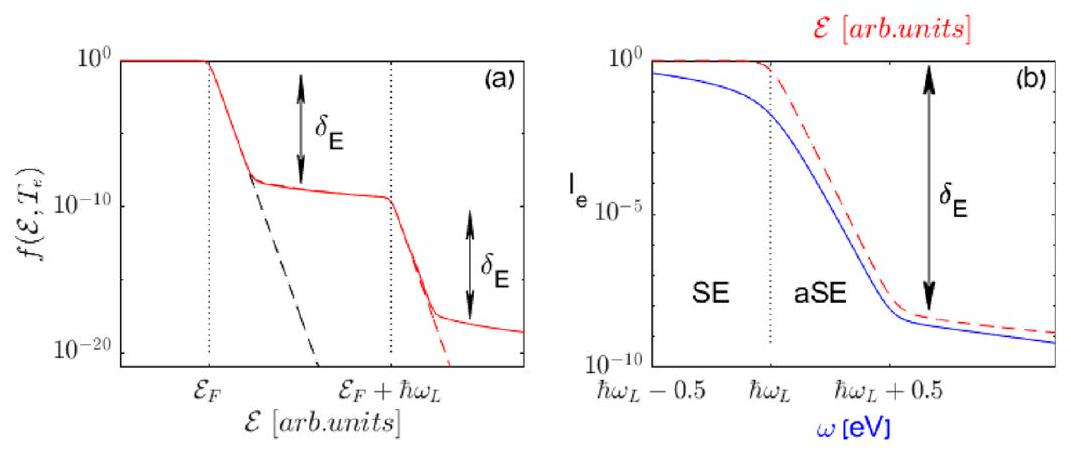
\includegraphics[alt={},max width=\textwidth]{f97508c2-190d-403e-b38d-02344f5e51bf-3_454_1071_226_550}
\captionsetup{labelformat=empty}
\caption{Figure 1. (Color online) (a) A typical nonequilibrium electron distribution $f(\mathcal{E})$ (3). Here, $\left|\hat{E}_{L}\right|^{2}=5 \times 10^{10}\left[V^{2} / m^{2}\right]$, $\hbar \omega_{L}=2.25 \mathrm{eV}$, and $\epsilon_{A g}= -8.5+1.8 i$. The theoretical prediction for the "hot" electron distribution (3) (red dashed line) is in excellent agreement with the full numerical result (red solid line). The thermal distribution at the steady-state electron temperature is shown by the dashed black line. (b) The electronic contribution to the emission (6) (blue solid line) compared to the distribution $f$ (3) (dashed red line).}
\end{center}
\end{figure}

briefly in the SI Section S2 for completeness. Here, we only recall how the nonthermal electron distribution (the solution of the Boltzmann equation (S11)) looks like, and describe several additional aspects of the solution which were not described before, but shall be important for the purpose of understanding the emission properties. Specifically, our examples hereafter consider a metal under CW illumination with a laser frequency $\hbar \omega_{L}=2.25 \mathrm{eV}$ and with a local field of I $\left.\hat{E}_{L}\right|^{2}=5 \times 10^{10} \mathrm{~V}^{2} / \mathrm{m}^{2}$. This value can be connected to the value of the incident intensity by specifying the geometry and material parameters; ignoring any near-field modification of the incident field, this value corresponds roughly to an incident intensity of $\sim 25 \mathrm{~kW} / \mathrm{cm}^{2}$ (as, e.g., in ref 23). All other parameters are the same as used in refs 3 and 52 .

In refs 3 and 52, it was shown that the nonequilibrium distribution near the Fermi energy obeys (to an excellent approximation) Fermi-Dirac statistics, namely, it is characterized by the proper steady-state electron temperature $T_{e}$ (which is higher (even if slightly) than the ambient temperature and determined by global energy conservation in the system). The main limitation of this solution is that near the Fermi energy the distribution is not exactly $f^{T}\left(\mathcal{E}, T_{e}\right)$ (see discussion in ref 3). However, for the purpose of the emission calculations, this small deviation is completely negligible.

Further away from the Fermi energy, the nonequilibrium is characterized by (relatively flat) $\hbar \omega_{L}$-wide shoulders, which represent the high energy nonthermal electrons (the so-called "hot" electrons, or "hot" carriers). Those were frequently incorrectly associated with faster chemical reactions (see discussion in refs 53, 56-58, 61, and 66 ; however, they are responsible for photodetection ${ }^{54,67-70}$ (and as shown below, also for the SE). Importantly, as the energy dependence of these nonthermal electrons does not resemble Fermi-Dirac statistics at all, there is no theoretical justification to attribute a temperature to them.

Since $e-p h$ interactions affect the electron distribution near the Fermi energy but are negligible further away from the Fermi energy, the probability of occupation in the "hot electrons shoulder" can be simply determined by balancing the $e-e$ collision term and the photon absorption term. ${ }^{52}$ This yields a simple approximation for the full nonequilibrium distribution

\[
\begin{array}{ll}
f\left(\mathcal{E}, T_{e} ;\left|\hat{E}_{L}\right|^{2}\right) & \cong f^{T}\left(\mathcal{E}, T_{e}\right)+\Delta f_{e}^{N T}+\Delta f_{h}^{N T} \\
\Delta f_{e}^{N T}\left(\mathcal{E}, T_{e} ;\left|\hat{E}_{L}\right|^{2}\right) & =\delta_{E} f^{T}\left(\mathcal{E}-\hbar \omega_{L}, T_{e}\right) \\
\Delta f_{h}^{N T}\left(\mathcal{E}, T_{e} ;\left|\hat{E}_{L}\right|^{2}\right) & =-\delta_{E} f^{T}\left(\mathcal{E}+\hbar \omega_{L}, T_{e}\right) \tag{3}
\end{array}
\]

where $\delta_{E}$ is a measure of the population inversion or the strength of the nonequilibrium. It is given by


\begin{align*}
\delta_{E} & \equiv\left|\frac{\hat{E}_{L}}{E_{s a t}}\right|^{2},\left|E_{s a t}\right|^{2} \equiv \frac{1}{\tau_{e-e} R}, \\
R & \equiv \frac{4 \epsilon_{0} \epsilon_{m}^{\prime \prime}\left(\omega_{L}\right)}{3 \hbar n_{e}} \frac{\mathcal{E}_{F}}{\hbar \omega_{L}}, \tag{4}
\end{align*}


where $\tau_{e-e}$ is the $e-e$ collision rate (appearing in the theory as part of the relaxation time approximation ${ }^{3}$ ), and $R$ is a constant that depends on the imaginary part of the metal permittivity at the laser frequency $\epsilon_{m}^{\prime \prime}$, Fermi energy $\mathcal{E}_{F}$, and electron density $n_{e}$ but not on $T_{e}$. Note that the corresponding expression in ref 52 had a small error; this is now pointed out in a correction, linked to that paper. $E_{\text {sat }}(4)$ is analogous to similar quantities appearing in the theory of atomic/molecular systems, e.g., in the context of lasing, but its value is significantly higher due to the rapid thermalization in metals; in ref 52, we showed that it roughly corresponds to $10^{11} \mathrm{~W} / \mathrm{cm}^{2}$.

The good agreement of the approximation (3) with the numerical solution of the Boltzmann equation (S11) can be seen in Figure 1a. The same calculations allow us to determine that the width of thermal regime is given by $\left.k_{B} T_{e} \log 1-\delta_{E}\right) / \delta_{E}$. This prediction improves upon the crude estimate in ref 71 and would be instrumental in aSE-based thermometry.

Figure 1a further shows that the distribution described above is "shifted and copied" to even higher electron energies, at a lowered occupation level. Specifically, beyond $\mathcal{E}_{F}+\hbar \omega_{L}$, the electron distribution decreases exponentially again such that the distribution is parallel to the thermal population but much higher. The distribution then settles to an additional (relatively flat) shoulder; a similar structure was observed for pulsed illumination ${ }^{72}$ but was not reported before for CW illumination. This, in fact, makes perfect sense because the distribution at $\mathcal{E}_{F}+\hbar \omega_{L}<\mathcal{E}<\mathcal{E}_{F}+2 \hbar \omega_{L}$ is generated via a (most likely, second) photon absorption by electrons in the regime $\mathcal{E}_{F}<\mathcal{E}<\mathcal{E}_{F}+\hbar \omega_{L}$. Considering again the competition between photon absorption and $e-e$ collisions, the\\
electron occupation in the regime $\mathcal{E}_{F}+\hbar \omega_{L}<\mathcal{E}<\mathcal{E}_{F}+2 \hbar \omega_{L}$ is simply a factor $\delta_{E}$ smaller than the corresponding occupation in the regime $\mathcal{E}_{F}<\mathcal{E}<\mathcal{E}_{F}+\hbar \omega_{L}$. Note that the second "hot" electron shoulder is not captured by the approximation (3). This can be straight-forwardly corrected (using additional higher-order terms) but is negligible for the purpose of emission calculations.

At this stage, it is important to note that the thermal part of the distribution $\left(f^{T}(\mathcal{E})\right)$ is much larger than the nonthermal part $\left( \pm \delta_{E} f^{T}\left(\mathcal{E} \mp \hbar \omega_{L}\right)\right)$ for energies close to the Fermi energy. However, it is much smaller than the nonthermal part within the "hot" carrier shoulder and beyond. This will be shown below to have important implications for the emission rate dependence on the incoming intensity.

Electronic Contribution to Emission. We now substitute the nonequilibrium distribution (3) in eq 1 to compute the "hot" PL. In order to obtain a simplified and physically insightful result, we evaluate the magnitude of the transition dipole moment and of the electron DOS at $\mathcal{E}=\mathcal{E}_{F}$. This approximation is expected to hold for Drude metals which are characterized by a smooth parabolic energy band. In this case, the emission integral simplifies to


\begin{equation*}
\Gamma^{e m}(\vec{r}, \omega)=\gamma_{\mathcal{E}}\left(\mathcal{E}_{F}, \vec{r}, \omega\right) \rho_{e}^{2}\left(\mathcal{E}_{F}\right) I_{e}\left(\omega, T_{e}\right) \tag{5}
\end{equation*}


where


\begin{equation*}
I_{e}\left(\omega, T_{e}\right)=\int f\left(\mathcal{E}+\hbar \omega, T_{e}\right)\left[\left(1-f\left(\mathcal{E}, T_{e}\right)\right] d \mathcal{E}\right. \tag{6}
\end{equation*}


represents the electronic part of the emission formula and


\begin{equation*}
\gamma_{\mathcal{E}}(\mathcal{E}, \vec{r}, \omega)=\frac{\pi \omega V_{N P}^{2}}{\epsilon_{0}}|\vec{\mu}(\mathcal{E}, \mathcal{E}+\hbar \omega)|^{2} \rho_{p h o t}(\vec{r}, \omega) \tag{7}
\end{equation*}


represents the emission rate of a single excited electron. The results presented below would change only marginally if the assumptions on the electron energy independence of the LDOPS and dipole moment are relaxed. This might be necessary, e.g., for few nm particles, which exhibit a nontrivial discrete energy spectrum; however, since the emission from such particles is weak (see e.g., refs 25 and 26 as well as below), this case is of lesser importance. As shall be shown, these simplifying assumptions enable simple and physically transparent analytic expressions for the emission rate to be attained.

For simplicity, and as frequently done in experimental studies, ${ }^{23,33}$ we first analyze the results without the LDOPS, i.e., we consider only $I_{e}$ (6). In Figure 1b, we plot $I_{e}(\omega)$ (6) and compare it to the distribution $f(\mathcal{E})$, revealing striking similarity. In particular, the regime of the emission curve below the laser frequency $\omega_{L}$ (aka the SE regime) is nearly flat, in similarity to the nonthermal electron shoulder. As shown in SI Section S3, this weak sensitivity to $\omega$ is related to the fact that the SE originates from the nonthermal part of the electron distribution which is nearly $\mathcal{E}$-independent.

In contrast, the low frequency part of the aSE (i.e., just above the laser frequency $\omega_{L}$ ) originates from the second thermal regime beyond $\mathcal{E}_{F}+\hbar \omega_{L}$ (see SI Section S3). Thus, if at all, it represents the electron temperature rather than the somewhat self-contradictory concept of nonthermal electron temperature (see ref 43). Similarly, the aSE should not be associated with the phonon temperature (see ref 50 ) even though it is nearly identical to the electron temperature. ${ }^{3}$ As a result, the spectral\\
dependence of the aSE in this specific segment resembles that of the BB emission, but it is far more intense; indeed, for temperatures not much higher than room temperature, the BB emission peaks in the mid infrared and has negligible intensity for visible frequencies; hence, it is not shown in Figure 1. Moreover, in contrast to the BB emission, this "thermal" segment of the emission curve extends only as much as the thermal regime of $f$.

Like the distribution, the low frequency part of the aSE is also terminated by a flat "shoulder", the relative height of which is similar to that of the "hot" electron shoulder in $f$, i.e., it is $\sim \delta_{E}$ times lower than the SE. As in the SE regime, this shoulder originates from the nonthermal electron part of the distribution (3), so that any attempt to extract a temperature from this spectral segment of the emission ${ }^{50}$ is bound to yield an unjustified, unrealistically high value.

Full Emission Spectra. The full emission spectra (the most accessible experimental observable) can be obtained by summing over the LDOPS for all emitter positions and multiplying it by $I_{e}(\omega)$ (6). This relies on the uniformity of the temperature inside metal nanoparticles. ${ }^{73,74}$ Thus, a theoretical prediction of the total emission from a given nanostructure requires the calculation of the LDOPS and the Green's tensor associated with it. This calculation is tedious unless it is done with an efficient modal method. ${ }^{75-77}$ As such a task is beyond the scope of the current work, we provide here only a qualitative discussion, focusing on the interplay between the laser frequency and the localized plasmon resonance (LPR) frequency; the latter is represented, following ref 78, by a somewhat-skewed Lorentzian, centered at $\omega_{L P R}$.

Figure 2a shows that the LDOPS determines the spectra only if $\omega_{L P R}<\omega_{L}$ (as, e.g., in ref 23 , where the laser wavelength

\begin{figure}[h]
\begin{center}
  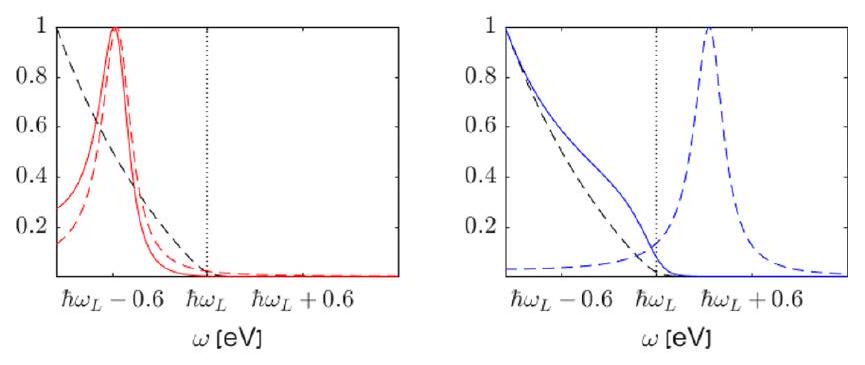
\includegraphics[alt={},max width=\textwidth]{f97508c2-190d-403e-b38d-02344f5e51bf-4_365_865_1487_1112}
\captionsetup{labelformat=empty}
\caption{Figure 2. (Color online) Normalized emission spectra for (1) $\hbar \omega_{L} =2.25 \mathrm{eV}$ and (a) $\omega_{L P R}=0.75 \omega_{L}$ and (b) $\omega_{L P R}=1.15 \omega_{L}$. The corresponding LDOPS are shown by dashed lines and $I_{e}(\omega)$ (6) is shown by a dashed black line.}
\end{center}
\end{figure}

was 532 nm and the (dipolar) LPR wavelength was $\sim 632 \mathrm{~nm}$ ), i.e., if the LPR frequency is in the SE regime; in this case, the electronic contribution only skews the spectrum slightly: it quenches the blue side and enhances the red side, but the overall overlap between the emission spectra and LDOPS is quite obvious. In this case, the emission from these modes would be proportional to the nanoparticle volume, as found experimentally in refs 25 and 26. However, when $\omega_{L P R}>\omega_{L}$ (LPR in the aSE region; a scenario which is more likely for higher-order modes), Figure 2 b shows that the electronic contribution $I_{e}(\omega)$ dominates the emission spectrum. In this case, since the slope of $I_{e}$ resembles the (electron) temperature, a sensitivity of the emission to that temperature is expected. Notably, however, this response could be probed only in the near-field because the higher-order modes associated with it

\begin{figure}[h]
\begin{center}
  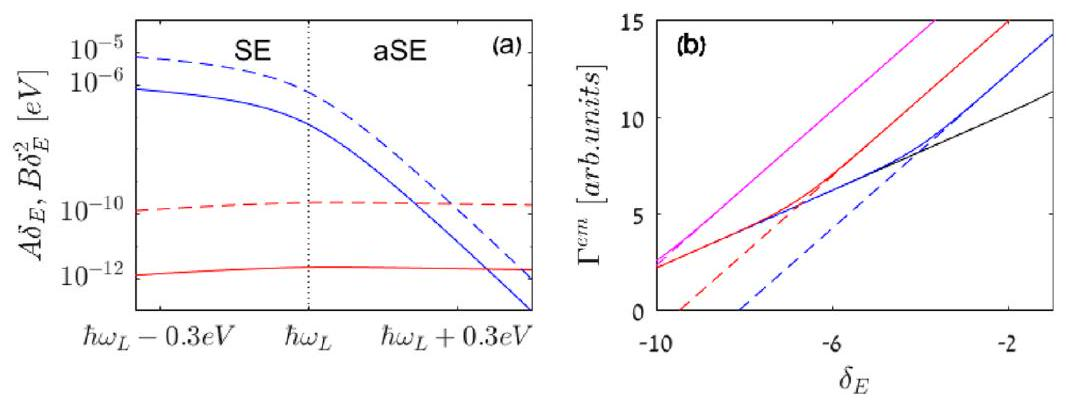
\includegraphics[alt={},max width=\textwidth]{f97508c2-190d-403e-b38d-02344f5e51bf-5_408_1067_228_552}
\captionsetup{labelformat=empty}
\caption{Figure 3. (Color online) (a) A comparison of $A(\omega) \delta_{E}$ (blue line) and $B(\omega) \delta_{E}^{2}$ (red line) for $\delta_{E}=10^{-6}$ (dashed) and $\delta_{E}=10^{-5}$ (solid). $A$ dominates except at the high frequency tail of the aSE. (b) Emission rate as a function of deviation from equilibrium $\delta_{E}$ for $\omega_{L}-0.4 \mathrm{eV}$ (black), $\omega_{L}+0.05 \mathrm{eV}$ (blue), $\omega_{L}+0.2 \mathrm{eV}$ (red), $\omega_{L}+0.4 \mathrm{eV}$ (magenta). The dashed lines are guides to the eye, demonstrating the change of slope of the emission curve for high illumination intensities.}
\end{center}
\end{figure}

are nonradiative and bound to the metal surface. As a result, the overall emission from these modes would be proportional to the surface area of the nanoparticle. All the above information sheds light on previous reports of the size and shape scaling of the emission.

Further Analysis. The dependence of the emission on the electron temperature $T_{e}$, the local electric field, and the laser frequency can be understood better via an approximate analytic solution of eq 5, obtained using the approximation (3). In the analysis below, we use for simplicity $\tau_{e-e}=$ Const (hence, $\delta_{E}=$ Const). It is given by


\begin{align*}
\Gamma^{e m}\left(\omega ; \omega_{L}, T_{e}\right)= & \gamma_{\mathcal{E}}\left(\mathcal{E}_{F}, \vec{r}, \omega\right) \rho_{e}^{2}\left(\mathcal{E}_{F}\right)\left[\left\langle\mathcal{E}_{B B}\left(\omega ; T_{e}\right)\right\rangle\right. \\
& \left.+A\left(\omega ; \omega_{L}, T_{e}\right) \delta_{E}+B\left(\omega ; \omega_{L}, T_{e}\right) \delta_{E}^{2}\right] \tag{8}
\end{align*}


where


\begin{align*}
& \left\langle\mathcal{E}_{B B}\left(\omega ; T_{e}\right)\right\rangle \approx \frac{\hbar \omega}{e^{\hbar \omega / k_{\mathrm{B}} T_{e}}-1} \\
& A\left(\omega ; \omega_{L}, T_{e}\right) \cong \frac{2 \hbar\left(\omega-\omega_{L}\right)}{e^{\hbar\left(\omega-\omega_{L}\right) / k_{\mathrm{B}} T_{e}}-1} \\
& B\left(\omega ; \omega_{L}, T_{e}\right) \cong-2 A\left(\omega ; \omega_{L}, T_{e}\right)+\frac{\hbar\left(\omega-2 \omega_{L}\right)}{e^{\hbar\left(\omega-2 \omega_{L}\right) / k_{\mathrm{B}} T_{e}}-1} \\
& =-2 A\left(\omega ; \omega_{L}, T_{e}\right)+\frac{1}{2} A\left(\omega ; 2 \omega_{L}, T_{e}\right) \tag{9}
\end{align*}


are parameters with units of energy and magnitude comparable to $\hbar \omega_{L}$. Here, we assumed that the temperature is much smaller than the width of the conduction band and that the laser and emission frequencies are within the optical range; the latter occurs when the temperatures are not much higher than room temperature: a condition which holds for practically all relevant scenarios, so that the approximation (8) is indistinguishable from the exact calculation.\\
$\left\langle\mathcal{E}_{B B}\right\rangle^{33}$ is the average energy of each electromagnetic mode with frequency $\omega$. ${ }^{79}$ Its product with $\gamma_{\mathcal{E}}$ represents the BB (i.e., ("standard") thermal) radiation which has been extensively studied in recent years in the context of LDOPS engineering. ${ }^{80-84}$ However, under the conditions specified above, in particular, for temperatures close to room temperature, this emission occurs mostly in the mid-IR, such that its contribution at optical frequencies is negligible compared with the next terms.

The next terms represent the "hot" PL due to one and two photon absorption, respectively. As expected (and shown explicitly in SI Section S3), they describe the deviation from the thermal emission (BB) and detailed balance considerations due to the nonthermal part of the electron distribution. Several conclusions can be drawn from their analytic form.

First, like $\left\langle\mathcal{E}_{B B}\right\rangle$, the parameters $A$ and $B$ depend on $\omega$ and on $T_{e}$; their dependence on $\omega_{L}$ involves just a shift. Thus, $A$ and $B$ primarily contain information about the Fermion statistics, i.e., their value is generic to all (Drude) metals. In that sense, the different emission characteristics of different materials, different structures, or different illumination conditions is incorporated only via $\delta_{E}$ and the LDOPS.

Second, the emission rate (8) does not follow exactly the Planck law (which reflects the boson statistics obeyed by the photons and detailed balance considerations) but rather a more complicated behavior which consists of several Plancklike terms. As previously assumed in the context of aSE-based thermometry, ${ }^{21-23}$ the second $(A)$ term in eq 8 includes a Planck-like term (at a shifted frequency), but the full expression includes also a (previously absent) factor $\omega-\omega_{L}$ in the numerator as well as two additional terms of higherorder in the electric field.

In order to elucidate this dependence, and the relative importance of the various terms in eq 8, we plot $A \delta_{E}$ vs $B \delta_{E}^{2}$ in Figure 3a. One can see that for the SE, $B \delta_{E}^{2}$ is negligible with respect to $A \delta_{E}$ whereas for the aSE, $B \delta_{E}^{2}$ becomes dominant above some threshold frequency, relatively far from $\omega_{L}$, such that it might be hard to access experimentally. This happens because of the above-mentioned dominance of $\Delta f_{e, h}^{N T}$ (the deviation from equilibrium) over the thermal distribution $f^{T}$ away from the Fermi energy; see eq 3 and the discussion that follows it. The crossover frequency decreases for increasing illumination intensity.

Third, the overall dependence of the emission spectrum on the electron temperature is weak for the SE (at least in the absence of the thermo-optic nonlinearity that affects the level of the local electric field ${ }^{85-87}$ ) but is important for the aSE tail of $A$.

Lastly, in analogy to the emission from molecules near plasmonic nanostructures, ${ }^{88,89}$ the emission rate scales as the product of the square of the local field with the LDOPS, i.e., $\rho_{\text {phot }}(\omega)\left|\hat{E}_{L}\right|^{2}$. This dependence is common to all emission processes ${ }^{7,8}$ and in particular to Raman scattering which was shown to be qualitatively similar to "hot" PL, even though quantitatively different. ${ }^{47}$ For sufficiently high illumination intensities, an additional term, proportional to $\left|\hat{E}_{L}\right|^{4}$, arises as\\
well, again, in similarity to Raman emission from molecules. ${ }^{90}$ In that context, it is important to clarify a potential confusion (see, e.g., ref 35): neglecting the difference between the absorbed and emitted frequencies ${ }^{91}$ and assuming the LDOPS scales as $\left|\hat{E}_{L} / E_{0}\right|^{2}$ allow showing that the Raman emission scales as the fourth power (i.e., to have a quartic scaling) with the electric field enhancement (i.e., with the local field normalized by the incident field) but to scale as the second power (quadratically) with the field itself; in contrast, the (additional) quartic dependence in the current context is genuinely with the field itself. This dependence necessarily originates from 2 photon absorption (regardless of the illumination intensity). As such, it is negligible for SE but non-negligible for the aSE. To see this more clearly, in Figure 3b, we plot the emission rate (1) as a function of the nonequilibrium strength parameter $\delta_{E}$ for several emission frequencies. One can see that the SE scales as $\left|\hat{E}_{L}\right|^{2}$, whereas the aSE scales as $\left|\hat{E}_{L}\right|^{4}$ (at least beyond some threshold nonequilibrium level). This analysis improves upon the power law scaling assumed in ref 43 which may have captured the transition region between the quadratic and quartic behaviors. Further nonlinearity may be observed for higher intensities, where the field-dependence of the temperature becomes of importance ${ }^{33,85-87}$ as that already observed in graphene. ${ }^{92}$ This regime and its relevance for the extraction of the electron temperature from the $\mathrm{aSE}^{21-24}$ will be explored in the future.

\section*{CONCLUSIONS}
Our results resolve a series of open questions associated with the nature of light emission from metals. First, they explain the similarity of the "hot" PL to BB emission ("thermal" PL) but also the numerous difference between them, namely, the limited extent of the spectral regime which resembles the BB emission and the much higher intensity of the "hot" PL. They also show that the emission does not follow Fermi-Dirac statistics; as it turns out, it also deviates from the BoseEinstein (Planck) statistics and detailed balance considerations (which determine the purely thermal blackbody emission). This resolves the disagreements about the "emission statistics" which arose in the context of thermometry techniques that were proposed recently. ${ }^{21-23}$

These techniques are related to a second open question, namely, the relation of the emission to the electron and phonon temperatures in the illuminated metal. For example, it was not clear whether the temperature extracted from the aSE in refs $21-24,42$, and 93 relates to the electron or phonon temperatures, or sometimes even to the self-contradictory concept of "non-thermal electron temperature". ${ }^{43,50}$ Our results show that the emission is primarily related to the electron temperature, yet its extraction may be more involved than that assumed so far (see also discussion in SI Section S3), especially in the presence of interband transitions.

In that context, the even higher frequency (flatter) part of the emission curve (similar to the one in Figure 1 b ) was sometimes associated with the phonon temperature or with a "hot" electron temperature. However, as it is difficult to retrieve from a single NP an aSE signal more than 2 orders of magnitude above the noise level (e.g., refs 5,23 , and 24 ), one may conclude that even when the signal was collected from a relatively large illuminated structure, the "shoulders" observed in Figure 2a of refs 50 and 51 may be experimental noise (rather than the signature of nonthermal electrons, in line with the speculation in ref 51); further support to this conclusion\\
may originate from the fact that the width of the thermal regime found in refs 23,24 , and 50 was much narrower compared with that of our prediction. Alternatively, the "shoulder" may have originated from interband transitions (which are not accounted for in our theory ${ }^{3}$ ) or another yet unidentified mechanism. Until this issue is clarified, the various temperatures extracted in those studies should be taken with a grain of salt.

In combination with a detailed knowledge of the spatial average of the LDOPS, the theory presented in this manuscript would enable a comparison to experimental data of "hot" PL from Ag NPs (e.g., ref 29) and thus, to the better understanding of the emission line shape. Note that in order to provide a quantitative prediction of the emission from metals, one needs also to know the transition matrix element and its energy dependence; those can be calculated from electron wave function calculations as, e.g., in refs 63, 64, and 94 or from more advanced DFT calculations (e.g., refs 95 and 96).

While our theory is so far limited to intraband transitions in Drude metals, there are various theoretical ${ }^{63,64}$ and experimental ${ }^{33}$ indications that imply that they are relevant also in the presence of some interband transitions. This can be verified upon extension of the underlying electronic theory ${ }^{3}$ to include also interband transitions in which case the theory of the current paper would be extended also to "hot" PL from other metals (Au, TiN, Cu, ...) and to emission at higher frequencies from Ag. In these cases, two photon absorption may be playing a more significant role, as it may enable otherwise inaccessible transitions such that it would be necessary to disentangle it from the two photon absorption signature emerging from the aSE (see Figure 3b). Such a disentanglement would be necessary also when our approach would be applied to transient PL (following an intense short pulse) ${ }^{33,62,65}$ and for high temperature PL. Thus, we conclude that the current study should be regarded only as the first act of a much deeper investigation into a much debated fundamental problem in solid-state and optical physics.

\section*{METHODS}
The spontaneous emission rate is calculated within the Fermi Golden Rule approximation ref 79 given by


\begin{equation*}
\left.R^{e m, i}(\vec{r}, \omega)=\frac{2 \pi}{\hbar} \sum_{f}|\langle f| \mathcal{H}(\vec{r}, \omega)| i\right\rangle\left.\right|^{2} f\left(\mathcal{E}_{i}\right)\left[1-f\left(\mathcal{E}_{f}\right)\right] \delta\left(\mathcal{E}_{f}-\mathcal{E}_{i}+\hbar \omega\right) \tag{10}
\end{equation*}


where $\langle f|$ is the final quantum state of the whole system (not to be confused with $f$, the (nonequilibrium) electron distribution function); it includes both the final electronic state as well as the emitted photon state (i.e., its frequency $\omega$ and modal indices $n, l, m$; notation associated with other properties, such as polarization, wavevector, is suppressed); in addition, $\mathcal{H} \equiv \hat{\mu} \cdot \vec{E}^{\wedge}(\vec{r}, \omega)$ is the electric dipole operator, with $\vec{E}^{\wedge}(\vec{r}, \omega)$ being the emitted (only!) electric field and $\hat{\mu} \sim \vec{\mu}\left(\mathcal{E}_{i}, \mathcal{E}_{f}\right) \sim q_{e}\langle f| \hat{\mu}|i\rangle$ the transition dipole moment operator. After some manipulation (see SI Section S1), this leads directly to eq 1.

In order to evaluate the nonequilibrium distributions, we solve the Boltzmann equation,


\begin{equation*}
\frac{\partial f\left(\mathcal{E} ; T_{e}, T_{p h}\right)}{\partial t}=\underbrace{\left(\frac{\partial f}{\partial t}\right)}_{\text {photonabsorption }}+\underbrace{\left(\frac{\partial f}{\partial t}\right)}_{e-\text { phcollisions }}+\underbrace{\left(\frac{\partial f}{\partial t}\right)}_{e-\text { ecollisions }} \tag{11}
\end{equation*}


where $f$ is the electron distribution function at an energy $\mathcal{E}$, electron temperature $T_{e}$, and phonon temperature $T_{p h}$, representing the population probability of electrons in a system characterized by a continuum of states within the conduction band. The equation is then solved analytically following the procedure outlined in ref 52, as detailed in SI Section S2.

\section*{ASSOCIATED CONTENT}
\section*{(I) Supporting Information}
The Supporting Information is available free of charge at \href{https://pubs.acs.org/doi/10.1021/acsnano.1c00835}{https://pubs.acs.org/doi/10.1021/acsnano.1c00835}.

Fermi golden rule formulation of the field distribution due to light emission from metals; nonequilibrium electron distribution; joint density of of pair states for illuminated metals, including Figure S1 (PDF)

\section*{AUTHOR INFORMATION}
\section*{Corresponding Author}
Yonatan Sivan - School of Electrical and Computer Engineering, Ben-Gurion University of the Negev, Be'er sheva, Israel 8410501; © \href{http://orcid.org/0000-0003-4361-4179;}{orcid.org/0000-0003-4361-4179;} Email: \href{mailto:sivanyon@bgu.ac.il}{sivanyon@bgu.ac.il}

\section*{Author}
Yonatan Dubi - Department of Chemistry, Ben-Gurion University of the Negev, Be'er sheva, Israel 8410501; © \href{http://orcid.org/0000-0002-8988-4935}{orcid.org/0000-0002-8988-4935}\\
Complete contact information is available at:\\
\href{https://pubs.acs.org/10.1021/acsnano.1c00835}{https://pubs.acs.org/10.1021/acsnano.1c00835}

\section*{Notes}
The authors declare no competing financial interest.

\section*{ACKNOWLEDGMENTS}
Y.S. was supported by Israel Science Foundation (ISF) grant (340/20) and MWK Niedersachsen funded project no. 76251-99-7/20 (ZN 3637). The authors would like to acknowledge many useful conversations with I.W. Un, M. Caldarola, and M. Orrit.

\section*{REFERENCES}
(1) Mooradian, A. Photoluminescence of Metals. Phys. Rev. Lett. 1969, 22, 185.\\
(2) Shen, Y. R. Distinction between Resonant Raman Scattering and Hot Luminescence. Phys. Rev. B 1974, 9, 622-626.\\
(3) Dubi, Y.; Sivan, Y. Hot electrons" in Metallic Nanostructures -Non-Thermal Carriers or Heating? Light: Sci. Appl. 2019, 8, 89.\\
(4) Apell, P.; Monreal, R.; Lundqvist, S. Photoluminescence of Noble Metals. Phys. Scr. 1988, 38, 174-179.\\
(5) Huang, J.; Wang, W.; Murphy, C. J.; Cahill, D. G. Resonant Secondary Light Emission from Plasmonic Au Nanostructures at High Electron Temperatures Created by Pulsed-Laser Excitation. Proc. Natl. Acad. Sci. U. S. A. 2014, 111, 906-911.\\
(6) Klein, M. V. Equivalence of Resonance Raman Scattering in Solids with Absorption Followed by Luminescence. Phys. Rev. B 1973, 8, 919-921.\\
(7) Solin, J. R.; Merkelo, H. Resonant Scattering or Absorption followed by Emission. Phys. Rev. B 1975, 12, 624-629.\\
(8) Solin, J. R.; Merkelo, H. Reply to "Comment on 'Resonant Scattering or Absorption Followed by Emission"'. Phys. Rev. B 1976, 14, 1775-1776.\\
(9) Shen, Y. R. Comment on "Resonant Scattering or Absorption Followed by Emission. Phys. Rev. B 1976, 9, 1772-1774.\\
(10) Boyd, G. T.; Yu, Z. H.; Shen, Y. R. Photoinduced Luminescence from the Noble Metals and its Enhancement on

Roughened Surfaces. Phys. Rev. B: Condens. Matter Mater. Phys. 1986, 33, 7923.\\
(11) Wilcoxon, J. P.; Martin, J. E.; Parsapour, F.; Wiedenman, B.; Kelley, D. F. Photoluminescence from Nanosize Gold Clusters. J. Chem. Phys. 1998, 108, 9137.\\
(12) Mohamed, M. B.; Volkov, V.; Link, S.; El-Sayed, M. A. The 'Lightning' Gold Nanorods: Fluorescence Enhancement of over a Million Compared to the Gold Metal. Chem. Phys. Lett. 2000, 317, 517-523.\\
(13) Huang, T.; Murray, R. W. Visible Luminescence of WaterSoluble Monolayer-Protected Gold Clusters. J. Phys. Chem. B 2001, 105, 12498-12502.\\
(14) Durr, N. J.; Larson, T.; Smith, D. K.; Korgel, B.; Sokolov, K.; Ben-Yakar, A. Two-Photon Luminescence Imaging of Cancer Cells Using Molecularly Targeted Gold Nanorods. Nano Lett. 2007, 4, 941-945.\\
(15) Wu, X.; Ming, T.; Wang, X.; Wang, P.; Wang, J.; Chen, J. High-Photoluminescence-Yield Gold Nanocubes: For Cell Imaging and Photothermal Therapy. ACS Nano 2010, 4, 113-120.\\
(16) Tcherniak, A.; Dominguez-Medina, S.; Chang, W.-S.; Swanglap, P.; Slaughter, L. S.; Landes, C. F.; Link, S. One-Photon Plasmon Luminescence and Its Application to Correlation Spectroscopy as a Probe for Rotational and Translational Dynamics of Gold Nanorods. J. Phys. Chem. C 2011, 115, 15938-15949.\\
(17) Zijlstra, P.; Chon, J. W. M.; Gu, M. A Five-Dimensional Optical Recording Mediated by Surface Plasmons in Gold Nanorods. Nature 2009, 459, 410.\\
(18) Zheng, Z.; Tachikawa, T.; Majima, T. Single-Particle Study of Pt-Modified Au Nanorods for Plasmon-Enhanced Hydrogen Generation in Visible to Near-Infrared Region. J. Am. Chem. Soc. 2014, 136, 6870-6873.\\
(19) Zheng, Z.; Tachikawa, T.; Majima, T. Plasmon-Enhanced Formic Acid Dehydrogenation Using Anisotropic Pd-Au Nanorods Studied at the Single-Particle Level. J. Am. Chem. Soc. 2015, 137, 948-957.\\
(20) Ghenuche, P.; Cherukulappurath, S.; Taminiau, T. H.; van Hulst, N. F.; Quidant, R. Spectroscopic Mode Mapping of Resonant Plasmon Nanoantennas. Phys. Rev. Lett. 2008, 101, 116805.\\
(21) Hugall, J. T.; Baumberg, J. J. Demonstrating Photoluminescence from Au is Electronic Inelastic Light Scattering of a Plasmonic Metal: The Origin of SERS Backgrounds. Nano Lett. 2015, 15, 2600-2604.\\
(22) Xie, X.; Cahill, D. G. Thermometry of Plasmonic Nanostructures by anti-Stokes Electronic Raman Scattering. Appl. Phys. Lett. 2016, 109, 183104.\\
(23) Carattino, A.; Caldarola, M.; Orrit, M. Gold Nanoparticles as Absolute Nano-Thermometers. Nano Lett. 2018, 18, 874-880.\\
(24) Jollans, T.; Caldarola, M.; Sivan, Y.; Orrit, M. Effective Electron Temperature Measurement Using Time-Resolved anti-Stokes Photoluminescence. J. Phys. Chem. A 2020, 124, 6968-6976.\\
(25) Dulkeith, E.; Niedereichholz, T.; Klar, T. A.; Feldmann, J.; von Plessen, G.; Gittins, D. I.; Mayya, K. S.; Caruso, F. Plasmon Emission in Photoexcited Gold Nanoparticles. Phys. Rev. B: Condens. Matter Mater. Phys. 2004, 70, 205424.\\
(26) Borys, N. J.; Walter, M. J.; Lupton, J. M. Intermittency in Second-Harmonic Radiation from Plasmonic Hot Spots on Rough Silver Films. Phys. Rev. B: Condens. Matter Mater. Phys. 2009, 80, 161407.\\
(27) Yorulmaz, M.; Khatua, S.; Zijlstra, P.; Gaiduk, A.; Orrit, M. Luminescence Quantum Yield of Single Gold Nanorods. Nano Lett. 2012, 12, 4385-4391.\\
(28) Fang, Y.; Chang, W. S.; Willingham, B.; Swanglap, P.; Dominguez-Medina, S.; Link, S. Plasmon Emission Quantum Yield of Single Gold Nanorods as a Function of Aspect Ratio. ACS Nano 2012, 6, 7177-7184.\\
(29) Lin, K.-Q.; Yi, J.; Hu, S.; Sun, J.-J.; Zheng, J.-T.; Wang, X.; Ren, B. Intraband Hot-Electron Photoluminescence from Single Silver Nanorods. ACS Photonics 2016, 3, 1248-1255.\\
(30) Eustis, S.; El-Sayed, M. Aspect Ratio Dependence of the Enhanced Fluorescence Intensity of Gold Nanorods: Experimental and Simulation Study. J. Phys. Chem. B 2005, 10, 16350-16356.\\
(31) Smitha, S. L.; Nissamudeen, K. M.; Philip, D.; Gopchandran, K. G. Studies on Surface Plasmon Resonance and Photoluminescence of Silver Nanoparticles. Spectrochim. Acta, Part A 2008, 71, 186-190.\\
(32) Yeshchenko, O. A.; Dmitruk, I. M.; Alexeenko, A. A.; Losytskyy, M. Y.; Kotko, A. V.; Pinchuk, A. O. Size-Dependent Surface-Plasmon Enhanced Photoluminescence from Silver Nanoparticles Embedded in Silica. Phys. Rev. B: Condens. Matter Mater. Phys. 2009, 79, 235438.\\
(33) Haug, T.; Klemm, P.; Bange, S.; Lupton, J. M. Hot-Electron Intraband Luminescence from Single Hot Spots in Noble-Metal Nanoparticle Films. Phys. Rev. Lett. 2015, 115, 067403.\\
(34) Beversluis, M.; Bouhelier, A.; Novotny, L. Continuum Generation from Single Gold Nanostructures through Near-Field Mediated Intraband Transitions. Phys. Rev. B: Condens. Matter Mater. Phys. 2003, 68, 115433.\\
(35) Mertens, J.; Kleemann, M.-E.; Chikkaraddy, R.; Narang, P.; Baumberg, J. J. How Light Is Emitted by Plasmonic Metals. Nano Lett. 2017, 17, 2568-2574.\\
(36) Bouhelier, A.; Bachelot, R.; Lerondel, G.; Kostcheev, S.; Royer, P.; Wiederrecht, G. P. Surface Plasmon Characteristics of Tunable Photoluminescence in Single Gold Nanorods. Phys. Rev. Lett. 2005, 95, 267405.\\
(37) Park, J.; Estrada, A.; Sharp, K.; Sang, K.; Schwartz, J. A.; Smith, D. K.; Coleman, C.; Payne, J. D.; Korgel, B. A.; Dunn, A. K.; Tunnell, J. W. Two-Photon-induced Photoluminescence Imaging of Tumors using Near-Infrared Excited Gold Nanoshells. Opt. Express 2008, 16, 1590.\\
(38) Sonnefraud, Y.; Sinclair, H. G.; Sivan, Y.; Foreman, M. R.; Dunsby, C.; Neil, M. A. A.; French, P. M.; Maier, S. A. Experimental Proof of Concept of Nanoparticle-Assisted STED. Nano Lett. 2014, 14, 4449-4453.\\
(39) Cortés, E.; Huidobro, P. A.; Sinclair, H. G.; Guldbrand, S.; Peveler, W. J.; Davies, T.; Parrinello, S.; Görlitz, F.; Dunsby, C.; Neil, M. A. A.; Sivan, Y.; Parkin, I. P.; French, P. M.; Maier, S. A. Plasmonic Nanoprobes for Stimulated Emission Depletion Microscopy. ACS Nano 2016, 10, 10454-10461.\\
(40) Hu, H.; Duan, H.; Yang, J. K. W.; Shen, Z. X. PlasmonModulated Photoluminescence of Individual Gold Nanostructures. ACS Nano 2012, 6, 10147-10155.\\
(41) Yin, T.; Dong, Z.; Jiang, L.; Zhang, L.; Hu, H.; Qiu, C.-W.; Yang, J. K. W.; Shen, Z. X. Anomalous Shift Behaviors in the Photoluminescence of Dolmen-Like Plasmonic Nanostructures. ACS Photonics 2016, 3, 979-984.\\
(42) Cai, Y.-Y.; Liu, J. G.; Tauzin, L. J.; Huang, D.; Sung, E.; Zhang, H.; Joplin, A.; Chang, W.-S.; Nordlander, P.; Link, S. Photoluminescence of Gold Nanorods: Purcell Effect Enhanced Emission from Hot Carriers. ACS Nano 2018, 12, 976-985.\\
(43) Cai, Y.-Y.; Sung, E.; Zhang, R.; Tauzin, L. J.; Liu, J. G.; Ostovar, B.; Zhang, Y.; Chang, W.-S.; Nordlander, P.; Link, S. Anti-Stokes Emission from Hot Carriers in Gold Nanorods. Nano Lett. 2019, 19, 1067-1073.\\
(44) Shahbazyan, T. V. Theory of Plasmon-Enhanced Metal Photoluminescence. Nano Lett. 2013, 13, 194-198.\\
(45) Portales, H.; Duval, E.; Saviot, L.; Fujii, M.; Sumitomo, M.; Hayashi, S. Raman Scattering by Electron-Hole Excitations in Silver Nanocrystals. Phys. Rev. B: Condens. Matter Mater. Phys. 2001, 63, 233402.\\
(46) Otto, A.; Akemann, W.; Pucci, A. Normal Bands in SurfaceEnhanced Raman Scattering (SERS) and Their Relation to the Electron-Hole Pair Excitation Background in SERS. Isr. J. Chem. 2006, 46, 307-315.\\
(47) Sun, G.; Khurgin, J. B.; Tsai, D. P. Comparative Analysis of Photoluminescence and Raman Enhancement by Metal Nanoparticles. Opt. Lett. 2012, 37, 1583.\\
(48) Manjavacas, A.; Liu, J. G.; Kulkarni, V.; Nordlander, P. Plasmon-Induced Hot Carriers in Metallic Nanoparticles. ACS Nano 2014, 8, 7630-7638.\\
(49) Liu, J. G.; Zhang, H.; Link, S.; Nordlander, P. Relaxation of Plasmon-Induced Hot Carriers. ACS Photonics 2018, 5, 2584-2595.\\
(50) Wu, S.; Hogan, N.; Sheldon, M. Hot Electron Emission in Plasmonic Thermionic Converters. ACS Energy Lett. 2019, 4, 25082513.\\
(51) Szczerbínski, J.; Gyr, L.; Kaeslin, G.; Zenobi, R. PlasmonDriven Photocatalysis Leads to Products Known from E-beam and X-ray-Induced Surface Chemistry. Nano Lett. 2018, 18, 6740-6749.\\
(52) Sivan, Y.; Un, I. W.; Dubi, Y. Assistance of Plasmonic Nanostructures to Photocatalysis - Just a Regular Heat Source. Faraday Discuss. 2019, 214, 215-233.\\
(53) Jain, P. K. Taking the Heat Off of Plasmonic Chemistry. J. Phys. Chem. C 2019, 123, 24347-24351.\\
(54) Xu, X.; Dutta, A.; Khurgin, J.; Wei, A.; Shalaev, V. M.; Boltasseva, A. TiN@TiO2 Core-Shell Nanoparticles as PlasmonEnhanced Photosensitizers: The Role of Hot Electron Injection. Laser Photonics Rev. 2020, 14, 1900376.\\
(55) Un, I. W.; Sivan, Y. The Role of Heat Generation and Fluid Flow in Plasmon-enhanced Reduction-Oxidation Reactions. ACS Photonics 2021,. 81183\\
(56) Sivan, Y.; Baraban, J.; Un, I. W.; Dubi, Y. Comment on "Quantifying Hot Carrier and Thermal Contributions in Plasmonic Photocatalysis". Science 2019, 364, No. eaaw9367.\\
(57) Sivan, Y.; Un, I. W.; Dubi, Y. Thermal Effects - an Alternative Mechanism for Plasmonic-Assisted Photo-catalysis. Chem. Sci. 2020, 11, 5017-5027.\\
(58) Sivan, Y.; Baraban, J.; Dubi, Y. Experimental Practices Required to Isolate Thermal Effects in Plasmonic Photo-catalysis - Lessons from Recent Experiments. OSA Continuum 2020, 3, 483-497.\\
(59) Un, I. W.; Sivan, Y. Parametric Study of Temperature Distribution in Plasmon-assisted Photocatalysis. Nanoscale 2020, 12, 17821-17832.\\
(60) Aizpurua, J.; Baletto, F.; Baumberg, J.; Christopher, P.; Nijs, B. d.; Deshpande, P.; Diaz Fernandez, Y.; Fabris, L.; Freakley, S.; Gawinkowski, S.; Govorov, A.; Halas, N.; Hernandez, R.; Jankiewicz, B.; Khurgin, J.; Kuisma, M.; Kumar, P. V.; Lischner, J.; Liu, J.; Marini, A.; et al. Theory of Hot Electrons: General Discussion. Faraday Discuss. 2019, 214, 245-281.\\
(61) Sivan, Y.; Dubi, Y. Recent Developments in Plasmon-Assisted Photocatalysis - a Personal Perspective. Appl. Phys. Lett. 2020, 117, 130501.\\
(62) Roloff, L.; Klemm, P.; Gronwald, I.; Huber, R.; Lupton, J. M.; Bange, S. Light Emission from Gold Nanoparticles under Ultrafast Near-Infrared Excitation: Thermal Radiation, Inelastic Light Scattering, or Multiphoton Luminescence? Nano Lett. 2017, 17, 7914-7919.\\
(63) Besteiro, L. V.; Kong, X.-T.; Wang, Z.; Hartland, G.; Govorov, A. O. Understanding Hot-Electron Generation and Plasmon Relaxation in Metal Nanocrystals: Quantum and Classical Mechanisms. ACS Photonics 2017, 4, 2759-2781.\\
(64) Khurgin, J. Hot Carriers Generated by plasmons: Where Are They Are Generated and Where Do They Go from There? Faraday Discuss. 2019, 214, 35-58.\\
(65) Agreda, A.; Sharma, D. K.; Viarbitskaya, S.; Hernandez, R.; Cluzel, B.; Demichel, O.; Weeber, J.-C.; des Francs, G. C.; Kumar, G. V. P.; Bouhelier, A. Spatial Distribution of the Nonlinear Photoluminescence in Au Nanowires. ACS Photonics 2019, 6, 1240-1247.\\
(66) Baffou, G.; Bordacchini, I.; Baldi, A.; Quidant, R. Simple Experimental Procedures to Discern Photothermal Processes in Plasmon-Driven Chemistry. Light: Sci. Appl. 2020, 9, 108.\\
(67) Goykhman, I.; Desiatov, B.; Khurgin, J.; Shappir, J.; Levy, U. Locally Oxidized Silicon Surface-Plasmon Schottky Detector for Telecom Regime. Nano Lett. 2011, 11, 2219-2224.\\
(68) Goykhman, I.; Desiatov, B.; Khurgin, J.; Shappir, J.; Levy, U. Waveguide based compact silicon Schottky photodetector with enhanced responsivity in the telecom spectral band. Opt. Express 2012, 20, 28594.\\
(69) Grajower, M.; Khurgin, J.; Levy, U. The Role of Surface Roughness in Plasmonic-Assisted Internal Photoemission Schottky Photodetectors. ACS Photonics 2018, 5, 4030-4036.\\
(70) Tagliabue, G.; Jermyn, A. S.; Sundararaman, R.; Welch, A. J.; DuChene, J. S.; Pala, R.; Davoyan, A. R.; Narang, P.; Atwater, H. A. Quantifying the Role of Surface Plasmon Excitation and Hot Carrier Transport in Plasmonic Devices. Nat. Commun. 2018, 9, 3394.\\
(71) Govorov, A. O.; Besteiro, L. V. Comments on ""Hot" Electrons in Metallic Nanostructures - Non-Thermal Carriers or Heating?" and "Assistance of Metal Nanoparticles to Photo-catalysis - Nothing More than a Classical Heat Source. ArXiv, \href{https://arxiv.org/abs/}{https://arxiv.org/abs/} 1906.06599 2019,.\\
(72) Pietanza, L. D.; Colonna, G.; Longo, S.; Capitelli, M. NonEquilibrium Electron and Phonon Dynamics in Metals under Femtosecond Laser Pulses. Eur. Phys. J. $D$ 2007, 45, 369-389.\\
(73) Baffou, G.; Quidant, R.; de Abajo, F. J. G. Nanoscale Control of Optical Heating in Complex Plasmonic Systems. ACS Nano 2010, 4, 709-716.\\
(74) Un, I. W.; Sivan, Y. Size-dependence of the Photothermal Response of a Single Metal Nanosphere. J. Appl. Phys. 2019, 126, 173103.\\
(75) Chen, P. Y.; Bergman, D. J.; Sivan, Y. Generalizing Normal Mode Expansion of Electromagnetic Green's Tensor to Lossy Resonators in Open Systems. Phys. Rev. Appl. 2019, 11, 044018.\\
(76) Rosolen, G.; Chen, P. Y.; Maes, B.; Sivan, Y. Overcoming the Bottleneck for Quantum Computations of Complex Nanophotonic Structures: Purcell and Förster Resonant Energy Transfer Calculations Using a Rigorous Mode-Hybridization Method. Phys. Rev. B: Condens. Matter Mater. Phys. 2020, 101, 155401.\\
(77) Chen, P. Y.; Sivan, Y. Resolving Gibbs Phenomenon via a Discontinuous Basis in a Mode Solver for Open Optical Systems. J. Comput. Phys. 2021, 429, 110004.\\
(78) Sauvan, C.; Hugonin, J. P.; Maksymov, I. S.; Lalanne, P. Theory of the Spontaneous Optical Emission of Nanosize Photonic and Plasmon Resonators. Phys. Rev. Lett. 2013, 110, 237401.\\
(79) Novotny, L.; Hecht, B. Principles of Nano-Optics; Cambridge University Press, Cambridge, 2006.\\
(80) Rodriguez, A. W.; Ilic, O.; Bermel, P.; Celanovic, I.; Joannopoulos, J.; Soljačić, M.; Johnson, S. Frequency-Selective Near-Field Radiative Heat Transfer between Photonic Crystal Slabs: A Computational Approach for Arbitrary Geometries and Materials. Phys. Rev. Lett. 2011, 107, 114302.\\
(81) Rodriguez, A. W.; Reid, M. T. H.; Johnson, S. G. Fluctuating-surface-current formulation of radiative heat transfer: Theory and applications. Phys. Rev. B: Condens. Matter Mater. Phys. 2013, 88, 054305.\\
(82) Guo, Y.; Jacob, Z. Thermal Hyperbolic Metamaterials. Opt. Express 2013, 21, 15014-15019.\\
(83) Dyachenko, P. N.; Molesky, S.; Petrov, A. Y.; Störmer, M.; Krekeler, T.; Lang, S.; Ritter, M.; Jacob, Z.; Eich, M. Controlling Thermal Emission with Refractory Epsilon-Near-Zero Metamaterials via Topological Transitions. Nat. Commun. 2016, 7, 2074-2080.\\
(84) Greffet, J.-J.; Bouchon, P.; Brucoli, G.; Marquier, F. Light Emission by Nonequilibrium Bodies: Local Kirchhoff Law. Phys. Rev. X 2018, 8, 021008.\\
(85) Sivan, Y.; Chu, S.-W. Nonlinear Plasmonics at High Temperatures. Nanophotonics 2017, 6, 317-328.\\
(86) Gurwich, I.; Sivan, Y. A Metal Nanosphere under Intense Continuous Wave Illumination - a Unique Case of Non-Perturbative Nonlinear Nanophotonics. Phys. Rev. E: Stat. Phys., Plasmas, Fluids, Relat. Interdiscip. Top. 2017, 96, 012212.\\
(87) Un, I. W.; Sivan, Y. The Thermo-Optic Nonlinearity of Single Metal Nanoparticles under Intense Continuous-Wave Illumination.\\
Phys. Rev. Mater. 2020, 4, 105201.\\
(88) Khurgin, J. B.; Sun, G.; Soref, R. A. Enhancement of Luminescence Efficiency using Surface Plasmon Polaritons: Figures of Merit. J. Opt. Soc. Am. B 2007, 24, 1968-1980.\\
(89) Khurgin, J. B.; Sun, G. Enhancement of Optical Properties of Nanoscaled Objects by Metal Nanoparticles. J. Opt. Soc. Am. B 2009, 26, B83.\\
(90) Zhang, Y.; Aizpurua, J.; Esteban, R. Optomechanical Collective Effects in Surface-Enhanced Raman Scattering from Many Molecules. ACS Photonics 2020, 7, 1676-1688.\\
(91) Le Ru, E. C.; Etchegoin, P. G. Principles of Surface-Enhanced Raman Spectroscopy and Related Plasmonic Effects; Elsevier, Amsterdam, 2009.\\
(92) Soavi, G.; Wang, G.; Rostami, H.; Tomadin, A.; Balci, O.; Paradisanos, I.; Pogna, E. A. A.; Cerullo, G.; Lidorikis, E.; Polini, M.; Ferrari, A. C. Hot Electrons Modulation of Third-Harmonic Generation in Graphene. ACS Photonics 2019, 6, 2841-2849.\\
(93) Jones, S.; André, D.; Karpinski, P.; Käll, M. Photothermal Heating of Plasmonic Nanoantennas: Influence on Trapped Particle Dynamics and Colloid Distribution. ACS Photonics 2018, 5, 28782887.\\
(94) Saavedra, J. R. M.; Asenjo-Garcia, A.; de Abajo, F. J. G. HotElectron Dynamics and Thermalization in Small Metallic Nanoparticles. ACS Photonics 2016, 3, 1637-1646.\\
(95) Brown, A. M.; Sundararaman, R.; Narang, P.; Goddard, W. A.; Atwater, H. A. Nonradiative Plasmon Decay and Hot Carrier Dynamics: Effects of Phonons, Surfaces, and Geometry. ACS Nano 2016, 10, 957-966.\\
(96) Forno, S. D.; Ranno, L.; Lischner, J. Material, Size and Environment Dependence of Plasmon-induced Hot Carriers in Metallic Nanoparticles. J. Phys. Chem. C 2018, 122, 8517-8527.


\end{document}